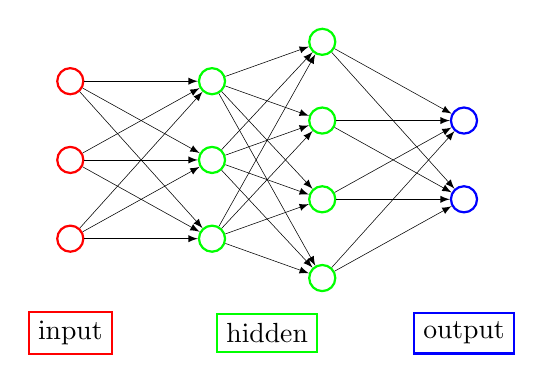
\begin{tikzpicture}
\usetikzlibrary{patterns}
\begin{scope}[very thin]
\foreach \x in {0, ..., 2} {
\node[circle, draw, color=red, thick] (input \x) at (-3, \x) {};
}
\foreach \x in {0, ..., 2} {
  \node[circle, draw, color=green, thick] (hidden1 \x) at (-1.2, \x) {};
  \foreach \y in {0,...,2}
    \draw[-latex] (input \y) -- (hidden1 \x);
}

\foreach \x in {0, ..., 3} {
  \node[circle, draw,color=green, thick] (hidden2 \x) at (0.2, \x-0.5) {};
  \foreach \y in {0, ..., 2}
    \draw[-latex] (hidden1 \y) -- (hidden2 \x);
}

\foreach \x in {0, ..., 1} {
  \node[circle, draw,color=blue, thick] (output \x) at (2, \x +0.5) {};
  \foreach \y in {0, ..., 3}
    \draw[-latex] (hidden2 \y) -- (output \x);
}

\node[rectangle, draw, color=red, text=black, thick] () at (-3, -1.2) {input};
\node[rectangle, draw, color=green, text=black, thick] () at (-.5, -1.2) {hidden};
\node[rectangle, draw, color=blue, text=black, thick]() at (2, -1.2) {output};
\end{scope}
\end{tikzpicture}